\documentclass[11pt, oneside]{article} 
\usepackage{geometry}
\geometry{letterpaper} 
\usepackage{graphicx}
	
\usepackage{amssymb}
\usepackage{amsmath}
\usepackage{parskip}
\usepackage{color}
\usepackage{hyperref}

\graphicspath{{/Users/telliott/Github/figures/}}
% \begin{center} \includegraphics [scale=0.4] {gauss3.png} \end{center}

\title{Ceva's theorem}
\date{}

\begin{document}
\maketitle
\Large

%[my-super-duper-separator]

There are some special points in triangles including orthocenters, which we've already mentioned, but also circumcenters, incenters and centroids.

They have the common feature that three lines are drawn crossing at a single point.  We need to establish the conditions under which this happens.

Begin with the triangle shown below, picking a point $P$ to be \emph{any point} inside the triangle.  Now draw line segments from each vertex through $P$ and extend them to the opposing side.
\begin{center} 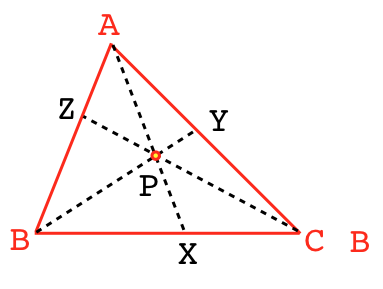
\includegraphics [scale=0.5] {Ceva1.png} \end{center}
Since $P$ can be anywhere, the ratio $BX/XC$ can be anything. Let's call it $x$.

\[ \frac{BX}{XC} = x \]

Line $AX$ divides the whole triangle into two parts.  

\begin{center} 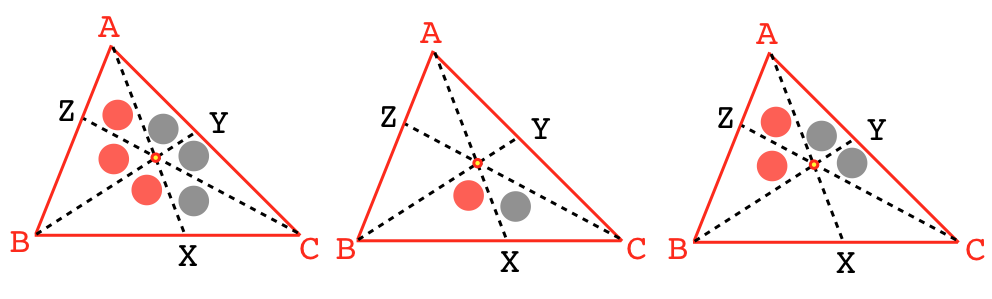
\includegraphics [scale=0.4] {Ceva2.png} \end{center}

We know that the area of $\triangle ABX$ is in the same proportion to the area of $\triangle AXC$ as $x$, because they share the same height, while $x$ is the ratio of their bases.  

\[ BX = x \cdot XC \]
\[ A_{ABX} = \frac{1}{2} h \cdot BX = \frac{1}{2} h \cdot x \cdot XC = x A_{AXC} \]

Now consider the lower pair of triangles $\triangle BPX$ and $\triangle CPX$ (middle panel).

These two also have their areas in the ratio $x$, for the same reason.
\begin{center} 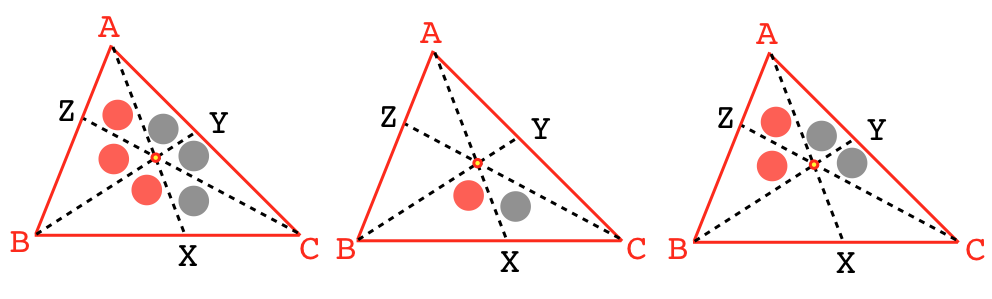
\includegraphics [scale=0.4] {Ceva2.png} \end{center}

By subtraction, $\triangle ABP$ and $\triangle ACP$ also have ratio $x$ (right panel).

So, altogether, we have that
\[ \frac{BX}{XC} = \frac{|ABX|}{|ACX|} = \frac{|BPX|}{|CPX|} = \frac{|ABP|}{|ACP|} = x \]

\subsection*{the other sides}

By the same reasoning, if $y=CY/YA$
\[ \frac{|BCP|}{|ABP|} = y \]
\begin{center} 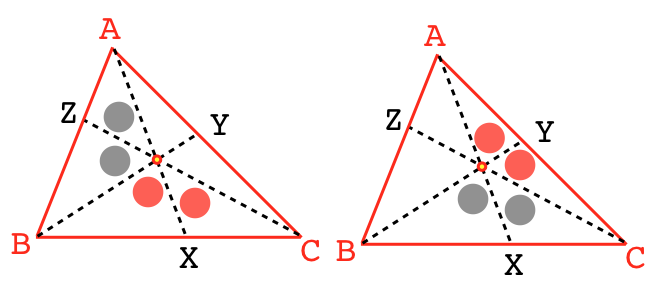
\includegraphics [scale=0.4] {Ceva3.png} \end{center}

and if $z= AZ/ZB$
\[ \frac{|ACP|}{|BCP|} = z \]

Now construct the product:

\[ xyz = \frac{|ABP|}{|ACP|} \ \frac{|BCP|}{|ABP|} \ \frac{|ACP|}{|BCP|} \]

But all terms cancel, so
\[ xyz = 1 \]
And this is of course true not just for the areas but for the original line segments
\[ xyz = \frac{BX}{XC} \ \frac{CY}{YA} \ \frac{AZ}{ZB} = 1 \]

$\square$

This proof also works in reverse,
\[ xyz = 1 \iff \text{3 lines cross at point P} \]

We will just assume that part.

\subsection*{orthocenter}

Consider this triangle in which we have drawn the altitudes to each side.  We claim that they cross at a single point, called the orthocenter.

\begin{center} 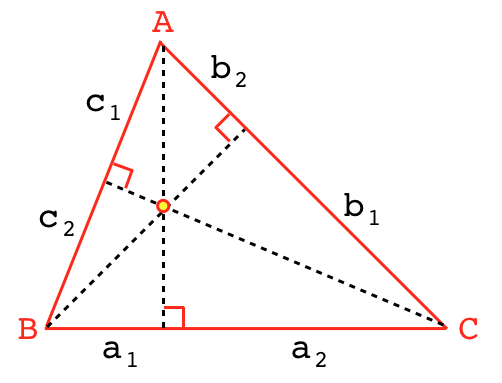
\includegraphics [scale=0.4] {ceva5.png} \end{center}

Let the angles be $A, B, C$ as labeled, and the sides opposite be $a, b, c$, subdivided as shown.

Then $\angle A$ is part of two right triangles, and by similar triangles we have that
\[ \frac{c_1}{b} = \frac{b_2}{c}, \ \ \ \ \ \ \frac{b_2}{c_1} = \frac{c}{b} \]

Similarly for $\angle B$
\[ \frac{a_1}{c} = \frac{c_2}{a}, \ \ \ \ \ \ \frac{c_2}{a_1} = \frac{a}{c} \]

And $\angle C$
\[ \frac{b_1}{a} = \frac{a_2}{b}, \ \ \ \ \ \ \frac{a_2}{b_1} = \frac{b}{a} \]

The product of ratios that we need is
\[ \frac{a_2}{a_1} \cdot \frac{b_2}{b_1} \cdot \frac{c_2}{c_1}  \]

Rearrange the denominators:
\[ \frac{a_2}{b_1} \cdot \frac{b_2}{c_1} \cdot \frac{c_2}{a_1}  \]

But these are the same ratios as we had above:
\[ = \frac{b}{a} \cdot \frac{c}{b} \cdot \frac{a}{c}  = 1 \]

\begin{center} 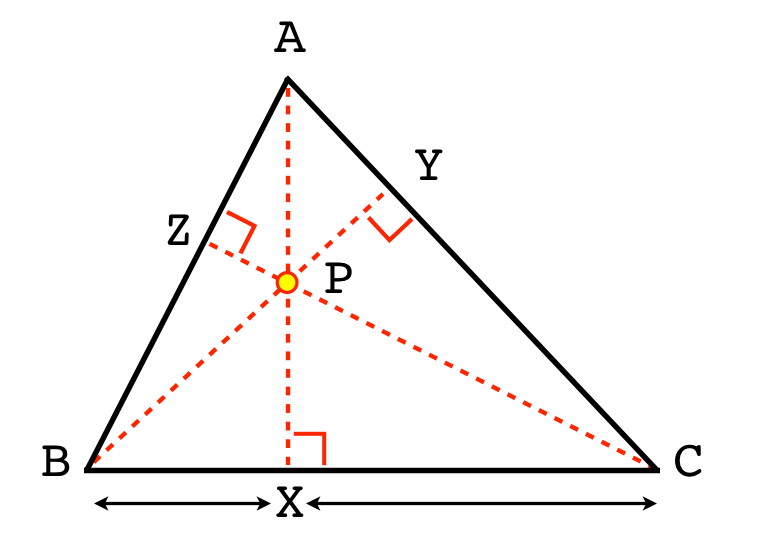
\includegraphics [scale=0.25] {ceva4.png} \end{center}

When we construct this product, all the terms cancel.

Therefore, the 3 altitudes all cross at a single point.  That point is the orthocenter, and this is a proof that it exists.

$\square$


\end{document}